\section{Data and methods}
\label{sec:datamethods}

\subsection{Data}
\label{subsec:data}
%TODO mention data acquisition in each section
%TODO table of data sets

	\begin{figure}[ht]
		\centering
		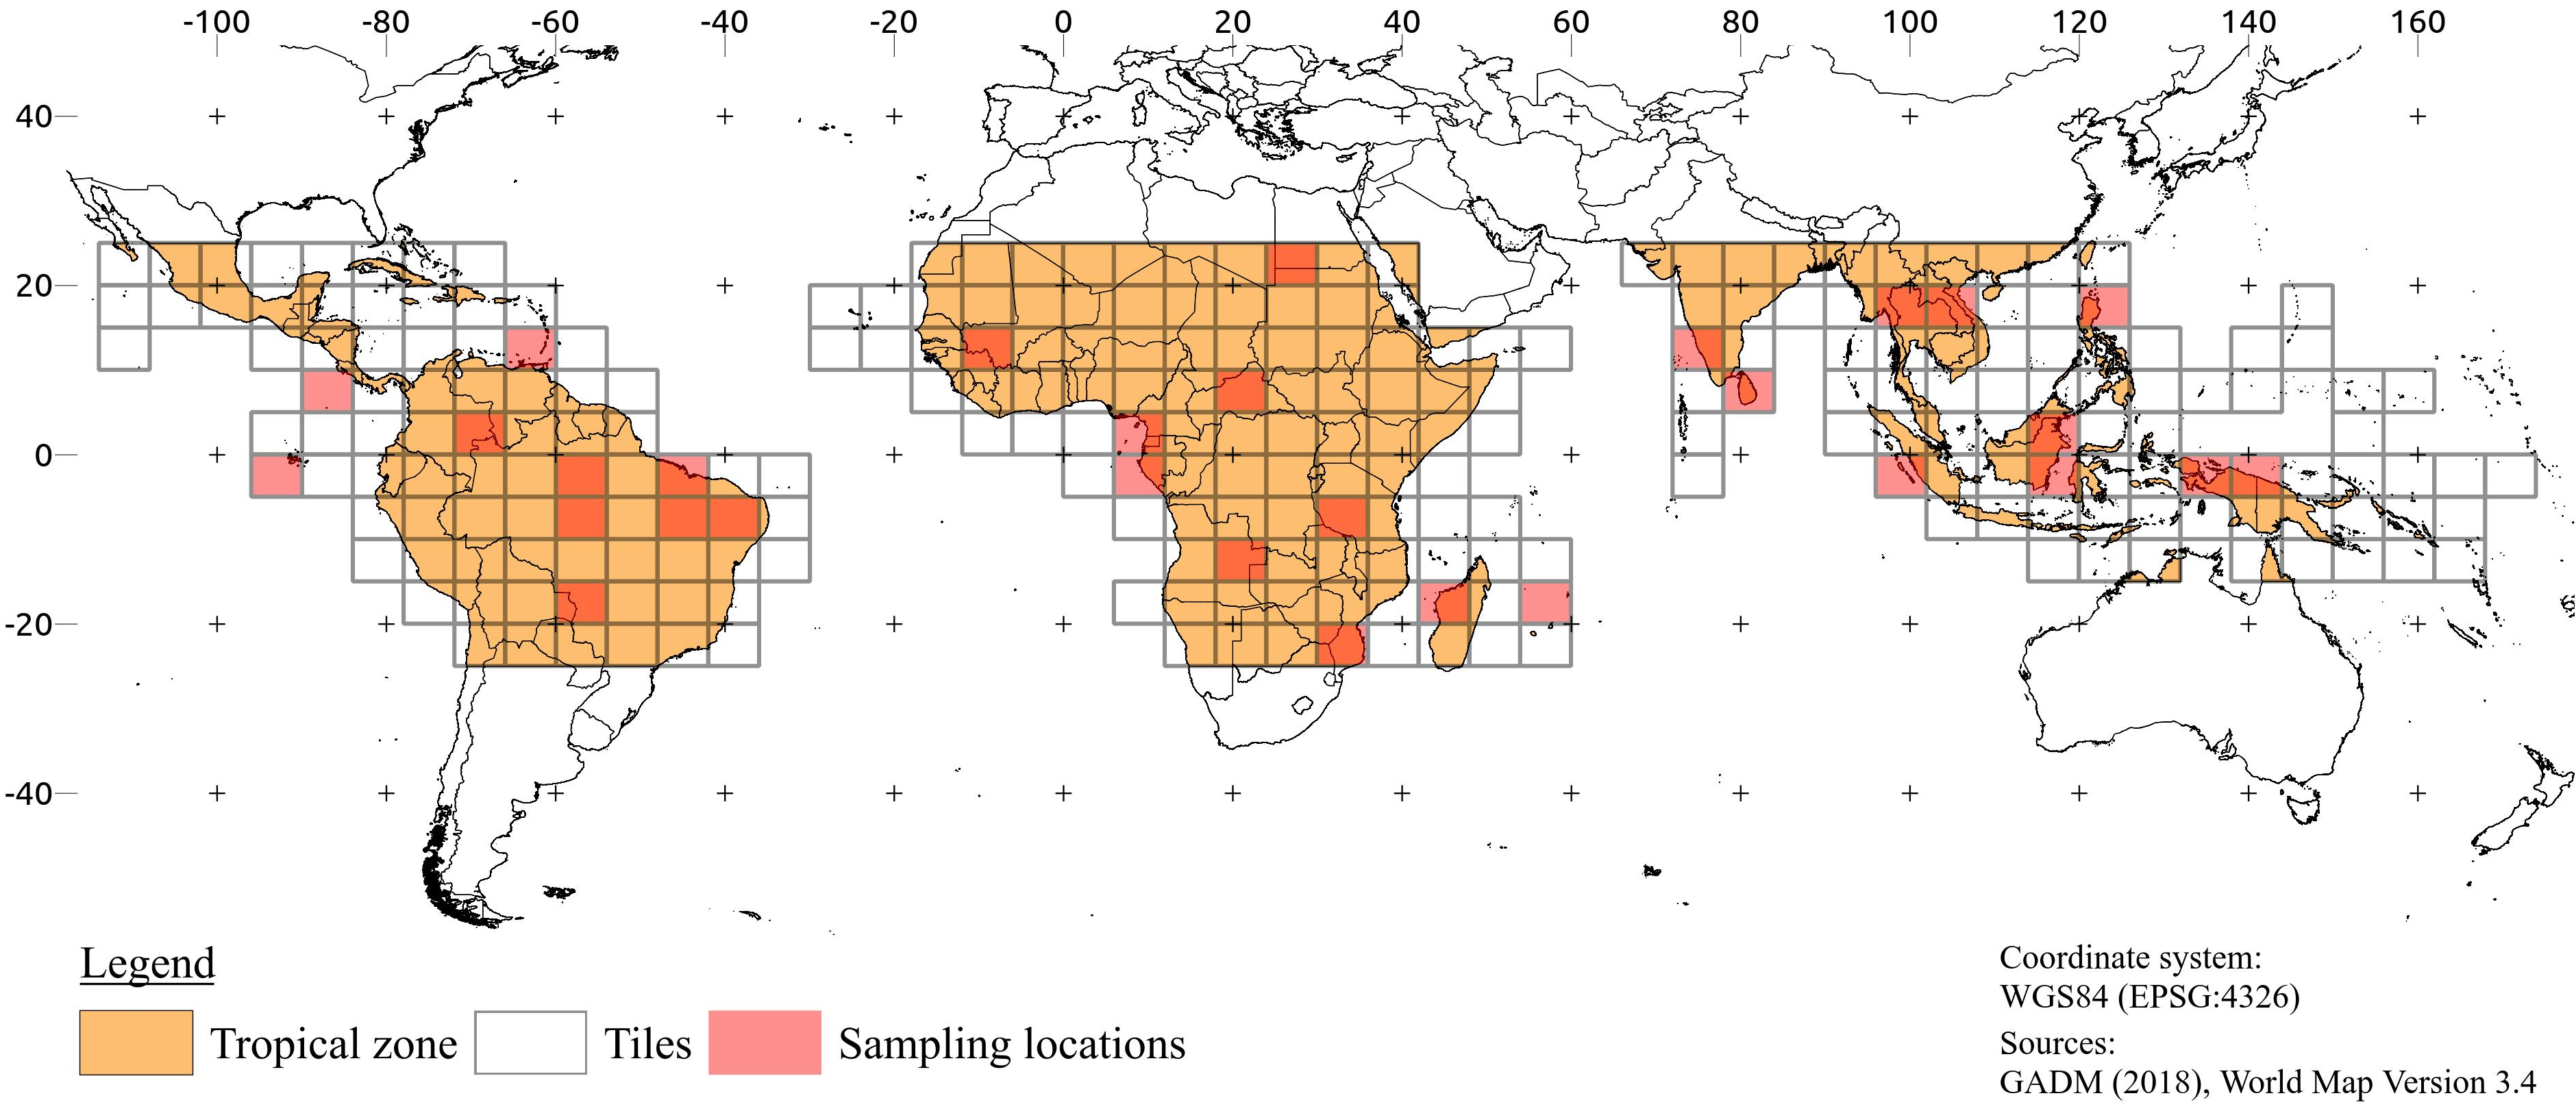
\includegraphics[scale=.97]{img/method_overview_frameless}
		\caption[Study extent]{Study extent and raster image tiles}
		\label{fig:studyextent}
	\end{figure}

	\subsubsection{Spatial data}
		\paragraph{Global Forest Change}
		\paragraph{GlobeLand30}
		\paragraph{Intact Forest Landscapes}
		\paragraph{Aboveground Woody Biomass}
		\paragraph{Global Soil Organic Carbon}
		\paragraph{Auxiliary}

	\subsubsection{Empirical data}
		\paragraph{Soil Organic Carbon}
		\paragraph{Ecosystem Service Values}


\subsection{Methods}
\label{subsec:methods}
%TODO need more speacking section headings
%TODO flowchart

	\subsubsection{Pre-processing}

	\subsubsection{Deforestation}
		\paragraph{Forest definition}
		\paragraph{Land use change driver}
		\paragraph{Accuracy assessment}

	\subsubsection{Emissions}
		\paragraph{Above ground biomass}
		\paragraph{Soil organic carbon change}

	\subsubsection{Ecosystem service values}
		\paragraph{Ecosystem service value loss}
		\paragraph{Ecosystem service value gain}

	\subsubsection{Binning analysis}